\documentclass[conference]{IEEEtran}
\usepackage{cite}
\usepackage{amsmath,amssymb}
\usepackage{graphicx}
\usepackage{booktabs}
\usepackage{url}
\graphicspath{{../outputs/figures/}}

\begin{document}
\title{Predictive Maintenance of Turbofan Engines: From Engineered Features to Deep Sequence Learning and Hybrid Fusion (Phase 2)}
\author{\IEEEauthorblockN{Sarvesh Choudhary, Arun Jangir, Keshav Chhabra, Mayank Yadav, Rohit Kumar}
\IEEEauthorblockA{\textit{Advanced Machine Learning and Deep Learning Capstone, Project 7: Remaining Useful Life Prediction}\\
Code: \url{https://github.com/Arunjangir8/Capstone_AML}}}

\maketitle
\begin{abstract}
Phase 1 of this project predicted the Remaining Useful Life (RUL) of turbofan engines on the NASA C-MAPSS FD001 subset with classical regressors trained on 71 hand-engineered degradation features; the best model, a Random Forest, reached a test RMSE of 11.44 cycles. Phase 2 removes the feature-engineering step: raw 30-cycle windows of 14 sensors are fed to a PyTorch Long Short-Term Memory (LSTM) network and a temporal 1D Convolutional Neural Network (1D-CNN). The LSTM reaches a test RMSE of 13.23 cycles without any engineered features, while the 1D-CNN reaches 18.93. A stage-wise error analysis shows that the two paradigms are complementary: the Random Forest is more accurate early in engine life, the LSTM close to failure. A hybrid that blends their predictions with a weight chosen on held-out validation engines ($w = 0.70$) achieves the best result on the official 100-engine test set: RMSE 10.99, MAE 7.98, $R^2$ 0.925 and NASA score 170.1.
\end{abstract}

\begin{IEEEkeywords}
Predictive maintenance, remaining useful life, C-MAPSS, LSTM, 1D-CNN, random forest, hybrid model
\end{IEEEkeywords}

\section{Introduction}
Unplanned failure of an aircraft engine is costly and dangerous, while replacing parts too early wastes useful life. Prognostics estimates the Remaining Useful Life (RUL): the number of operating cycles left before an engine reaches failure. Accurate RUL estimates let operators schedule maintenance just in time.

In Phase 1 we built a leakage-free pipeline on NASA C-MAPSS FD001 and trained Linear Regression, a Decision Tree and a Random Forest on 71 engineered features (rolling mean and standard deviation, trend slope, and deviation from the engine's healthy baseline). These features carried most of the signal: without them the Random Forest's validation RMSE rose from 10.34 to 15.98 cycles. Phase 2 asks whether deep sequence models can learn this degradation signal directly from raw sensor windows, how they compare with the Phase 1 models under identical conditions, and whether the two paradigms can be combined.

The contributions of Phase 2 are: (1) a sequence-windowing pipeline that reuses the Phase 1 engine split so results are directly comparable; (2) PyTorch LSTM and 1D-CNN regressors trained end-to-end on raw sensors; (3) a stage-wise comparison of Phase 1 and Phase 2 errors; and (4) a validation-tuned hybrid of the best model from each phase.


\section{Related Work}
Saxena \textit{et al.} introduced the C-MAPSS run-to-failure simulation and the asymmetric scoring function used here \cite{r1}. Classical data-driven approaches regress RUL from summary statistics of sensor windows. Deep learning approaches remove this step: Babu \textit{et al.} \cite{r3} and Li \textit{et al.} \cite{r5} applied convolutional networks to sensor windows, and Zheng \textit{et al.} \cite{r4} showed that LSTMs \cite{r2} capture the temporal dynamics of degradation. Our work compares both families on one pipeline and combines them.


\section{Dataset and Experimental Setup}
\subsection{C-MAPSS FD001}
FD001 contains 100 training engines run to failure (20,631 cycles) and 100 test engines whose records stop before failure, with the true RUL given separately. It has one operating condition and one fault mode (high-pressure compressor degradation). We keep the 14 sensors that vary over engine life (s2, s3, s4, s7, s8, s9, s11, s12, s13, s14, s15, s17, s20, s21).

\subsection{Target and Split}
The target is the piecewise-linear RUL capped at 125 cycles, as in Phase 1. Training engines are split 80/20 at engine level with GroupShuffleSplit (seed 42), so no engine appears in both training and validation. Both phases use exactly the same 80 training and 20 validation engines and the same official test set.

\subsection{Metrics}
We report RMSE, MAE and $R^2$ in cycles, and the NASA asymmetric score

\begin{equation}
S = \sum_{i} \begin{cases} e^{-d_i/13}-1, & d_i < 0 \\ e^{d_i/10}-1, & d_i \ge 0 \end{cases}, \quad d_i = \hat{y}_i - y_i
\label{eq1}
\end{equation}
which penalises late predictions (over-estimating remaining life) more heavily than early ones.


\section{Phase 2 Methodology}
\subsection{Sequence Construction}
Sensors are scaled to $[-1, 1]$ with a MinMaxScaler fitted on the 80 training engines only, then each engine is cut into sliding windows of $W = 30$ cycles. A window ending at cycle t is labelled with the capped RUL at t, and windows never cross engine boundaries. This yields 14,241 training and 3,490 validation windows of shape 30 $\times$ 14. Each test engine contributes its final 30 cycles (the shortest test record has 31 cycles, so no padding is needed). Fig. 1 contrasts a healthy and a degrading window.

\begin{figure}[!t]
\centering
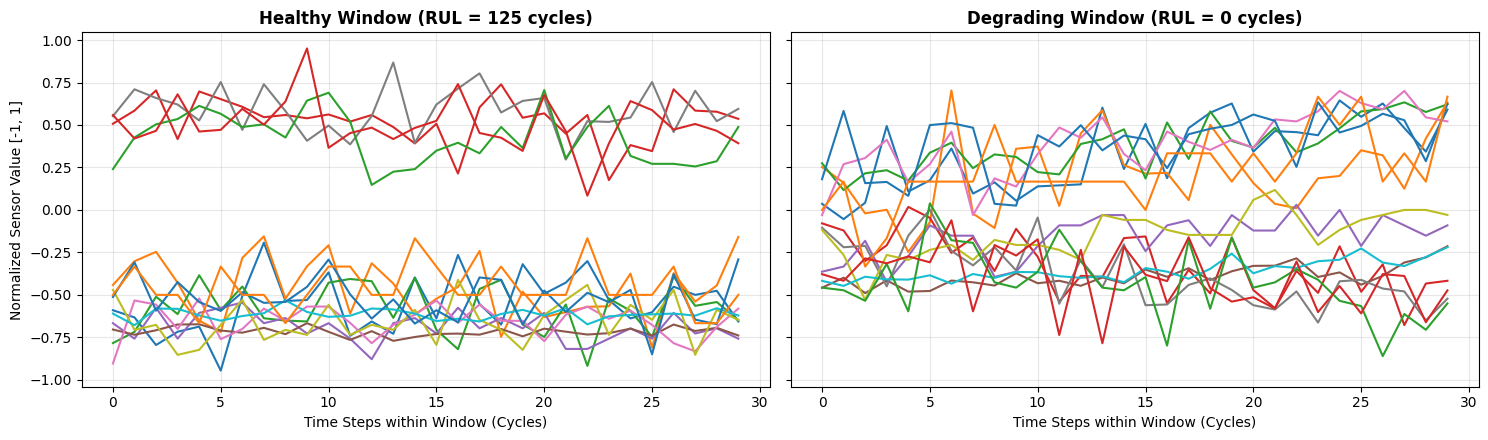
\includegraphics[width=\columnwidth]{07_sequence_window_visualization.png}
\caption{Normalised sensor values inside a 30-cycle window early in life (left, RUL = 125) and just before failure (right).}
\label{fig1}
\end{figure}

\subsection{LSTM Regressor}
The LSTM has two stacked layers with 64 hidden units and dropout 0.2. The final hidden state passes through a head Linear(64, 32), ReLU, Dropout(0.2), Linear(32, 1), giving 55,873 trainable parameters.

\subsection{Temporal 1D-CNN}
The 1D-CNN treats the 14 sensors as channels: Conv1d(14$\rightarrow$32, k=5) and Conv1d(32$\rightarrow$64, k=5), each with batch normalisation and ReLU, then max-pooling, Conv1d(64$\rightarrow$128, k=3), global average pooling and the same style of dense head.

\subsection{Training}
Both networks use Huber (Smooth L1) loss, AdamW (learning rate 0.002, weight decay 10$^{-4}$), batch size 64, ReduceLROnPlateau (factor 0.5, patience 3) and early stopping with patience 8 on validation loss, for at most 34 epochs. The LSTM stopped at epoch 12 and the 1D-CNN at epoch 24; the best validation weights are restored.

\subsection{Hybrid Fusion}
The hybrid combines the best model from each phase:

\begin{equation}
\hat{y}_{\mathrm{hyb}} = w\,\hat{y}_{\mathrm{RF}} + (1-w)\,\hat{y}_{\mathrm{LSTM}}
\label{eq2}
\end{equation}
The weight w is chosen by grid search over $[0, 1]$ in steps of 0.01 to minimise RMSE on the 3,490 validation windows, matched by engine and cycle across the two models. The selected weight is $w = 0.70$ (validation RMSE 10.50). The test set is used only for the final evaluation. The blend helps because the two models make different errors, as shown in Section VI.


\section{Results}
\subsection{Official Test Set}
Table I lists all models on the 100 official test engines. The LSTM, trained on raw sensors alone, beats both linear regression and the decision tree, which needed the 71 engineered features. It does not beat the Random Forest. The 1D-CNN is the weakest learned model; its validation loss oscillated during training and it over-predicts several engines near failure, which explains its large NASA score. The hybrid is best on all four metrics.

\begin{table}[!t]
\caption{Official FD001 test results (100 engines)}
\label{tabI}
\centering
\footnotesize
\begin{tabular}{lccccc}
\toprule
Model & Phase & RMSE & MAE & $R^2$ & NASA S \\
\midrule
Mean baseline & - & 51.63 & 39.47 & -0.660 & 248,340.7 \\
Linear Regression & 1 & 15.85 & 12.84 & 0.844 & 406.6 \\
Decision Tree & 1 & 14.96 & 10.80 & 0.861 & 357.0 \\
Random Forest & 1 & 11.44 & 8.27 & 0.918 & 184.5 \\
1D-CNN & 2 & 18.93 & 13.30 & 0.777 & 1,404.3 \\
LSTM & 2 & 13.23 & 9.88 & 0.891 & 240.5 \\
\textbf{Hybrid (RF + LSTM)} & 1+2 & \textbf{10.99} & \textbf{7.98} & \textbf{0.925} & \textbf{170.1} \\
\bottomrule
\end{tabular}
\end{table}

\begin{figure}[!t]
\centering
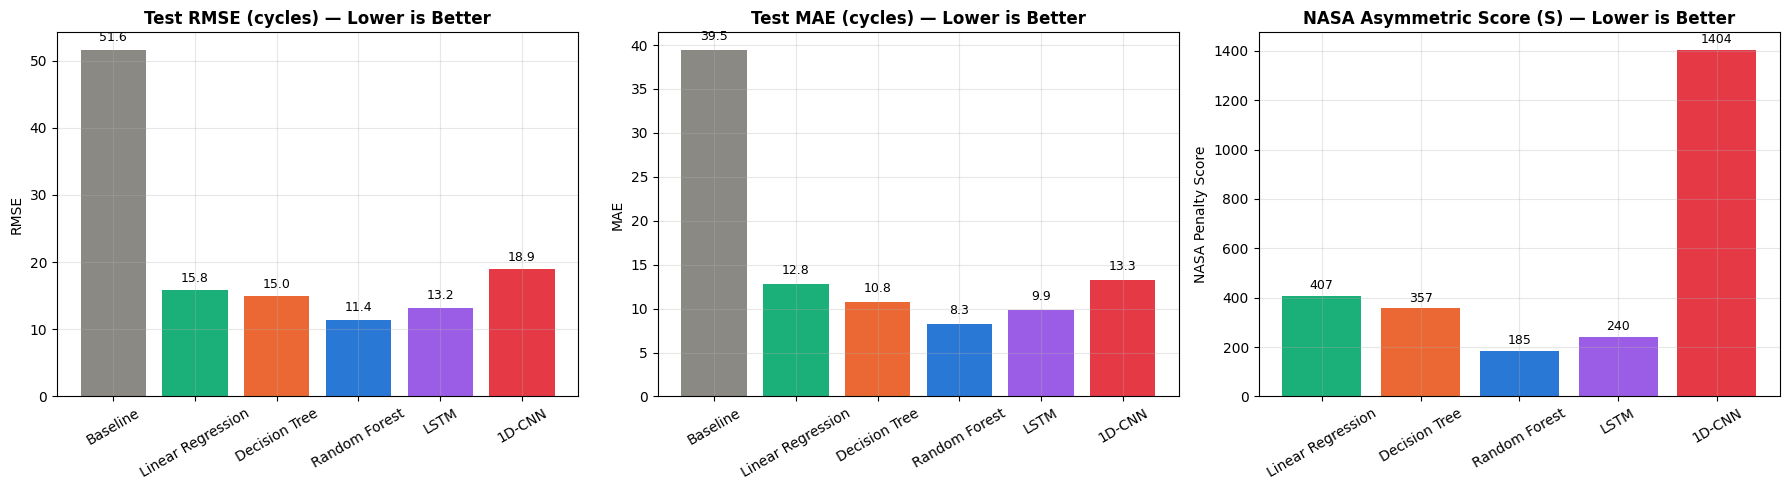
\includegraphics[width=\columnwidth]{10_phase1_vs_phase2_test_comparison.png}
\caption{Test RMSE, MAE and NASA score of the Phase 1 and Phase 2 models.}
\label{fig2}
\end{figure}

\begin{figure}[!t]
\centering
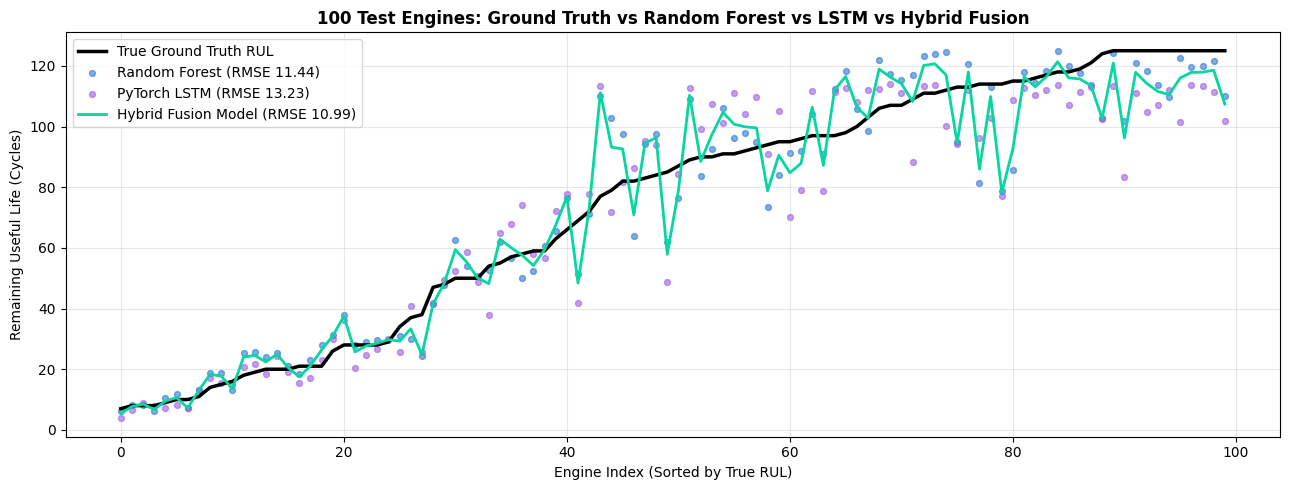
\includegraphics[width=\columnwidth]{11_hybrid_test_scatter.png}
\caption{Predictions on the 100 test engines sorted by true RUL: Random Forest, LSTM and the hybrid.}
\label{fig3}
\end{figure}


\section{Phase 1 versus Phase 2}
\subsection{Stage-wise Errors}
Table II splits the validation error by life stage. The Random Forest is clearly better in the early, healthy stage (RUL $>$ 100), where its baseline-deviation features detect that nothing has changed yet. The LSTM over-predicts degradation in this stage, but in the late stage (RUL $\le$ 100) it is slightly better than the Random Forest, and in the critical last 50 cycles it is better by 0.7 cycles. Because the errors differ by stage, blending them reduces late-stage RMSE from 12.26 to 10.84 cycles.

\begin{table}[!t]
\caption{Validation RMSE by life stage (3,490 windows)}
\label{tabII}
\centering
\footnotesize
\begin{tabular}{lccc}
\toprule
Model & Early ($>$100) & Late ($\le$100) & Critical ($\le$50) \\
\midrule
Random Forest & 9.33 & 12.26 & 6.58 \\
LSTM & 15.44 & 12.08 & 5.87 \\
\textbf{Hybrid} & 10.02 & \textbf{10.84} & \textbf{5.54} \\
\bottomrule
\end{tabular}
\end{table}

\subsection{Comparison of the Two Phases}
Table III summarises the practical differences. Phase 1 needs domain knowledge to design features but trains in seconds and is easy to interpret through feature importances. Phase 2 needs no feature design and is stronger near failure, at the cost of a fixed minimum history of 30 cycles, longer training and less interpretability. The hybrid keeps the strengths of both.

\begin{table}[!t]
\caption{Phase 1 and Phase 2 compared}
\label{tabIII}
\centering
\footnotesize
\begin{tabular}{lcc}
\toprule
Aspect & Phase 1 & Phase 2 \\
\midrule
Input & 71 engineered features per cycle & Raw 30 $\times$ 14 sensor window \\
Feature design & Manual, domain-driven & Learned end-to-end \\
Models & LR, Decision Tree, RF & LSTM, 1D-CNN, hybrid \\
Best test RMSE & 11.44 (RF) & 13.23 (LSTM); 10.99 (hybrid) \\
Stronger stage & Early life & Late life \\
Interpretability & High (importances) & Low \\
\bottomrule
\end{tabular}
\end{table}


\section{Limitations}
All experiments use FD001 only, which has a single operating condition and fault mode; FD002--FD004 remain to be tested. The hybrid uses one global weight; a stage-aware weight or a learned stacking model may do better. Sensitivity to the window length W and to the choice of loss function (MSE versus Huber) was planned but has not yet been run end-to-end, so $W = 30$ and Huber loss are design choices rather than tuned results. Each network was trained with a single seed.


\section{Conclusion}
Phase 2 showed that an LSTM can learn engine degradation from raw sensor windows without hand-crafted features, reaching a test RMSE of 13.23 cycles and outperforming two of the three Phase 1 models. Engineered features remain valuable: the Phase 1 Random Forest is still the best single model and is more accurate in early life. Fusing the two with a validation-tuned weight gives the best overall result, RMSE 10.99 cycles and NASA score 170.1, with the largest gains in the late stage where maintenance decisions are made.


\begin{thebibliography}{00}
\bibitem{r1} A. Saxena, K. Goebel, D. Simon, and N. Eklund, ``Damage propagation modeling for aircraft engine run-to-failure simulation,'' in \textit{Proc. Int. Conf. Prognostics and Health Management}, 2008, pp. 1--9.
\bibitem{r2} S. Hochreiter and J. Schmidhuber, ``Long short-term memory,'' \textit{Neural Computation}, vol. 9, no. 8, pp. 1735--1780, 1997.
\bibitem{r3} G. S. Babu, P. Zhao, and X.-L. Li, ``Deep convolutional neural network based regression approach for estimation of remaining useful life,'' in \textit{Proc. DASFAA}, 2016, pp. 214--228.
\bibitem{r4} S. Zheng, K. Ristovski, A. Farahat, and C. Gupta, ``Long short-term memory network for remaining useful life estimation,'' in \textit{Proc. IEEE Int. Conf. Prognostics and Health Management}, 2017, pp. 88--95.
\bibitem{r5} X. Li, Q. Ding, and J.-Q. Sun, ``Remaining useful life estimation in prognostics using deep convolution neural networks,'' \textit{Reliability Engineering \& System Safety}, vol. 172, pp. 1--11, 2018.
\end{thebibliography}

\end{document}
